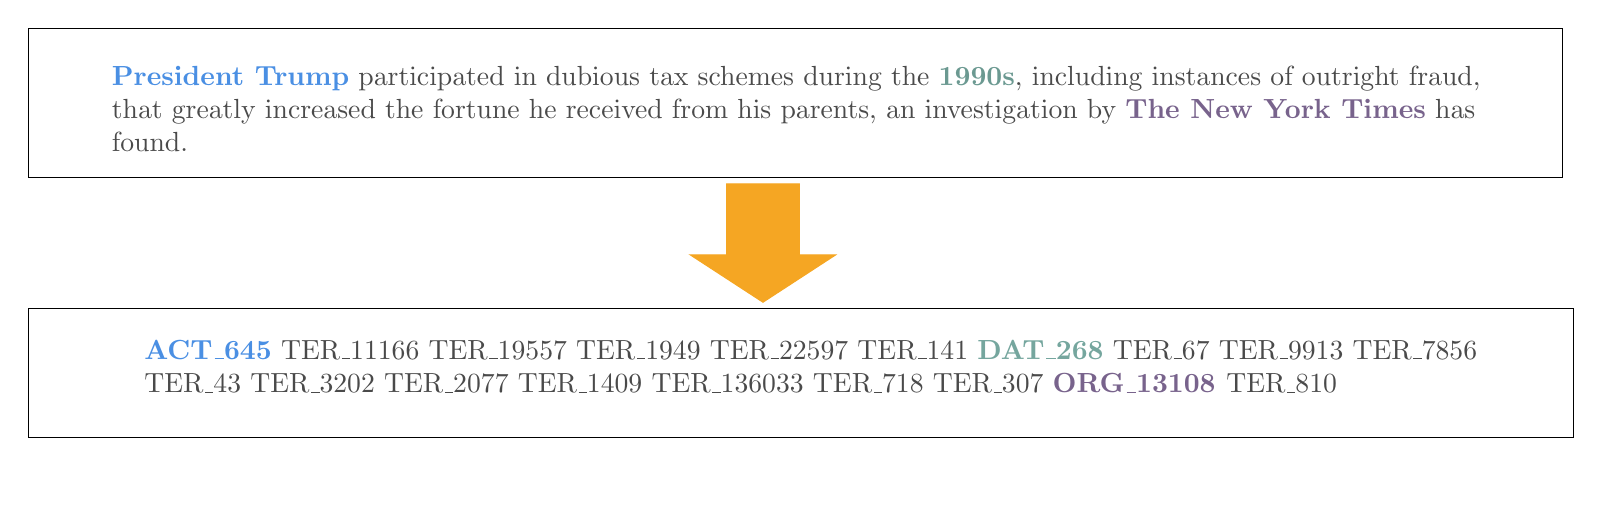
\begin{tikzpicture}[x=0.75pt,y=0.75pt,yscale=-1,xscale=1]
%uncomment if require: \path (0,377); %set diagram left start at 0, and has height of 377

%Shape: Rectangle [id:dp8906489990544584] 
\draw   (28,17) -- (767,17) -- (767,89) -- (28,89) -- cycle ;
%Shape: Rectangle [id:dp9074920271044917] 
\draw   (28,152) -- (772.5,152) -- (772.5,214) -- (28,214) -- cycle ;
%Down Arrow [id:dp1838486332286331] 
\draw  [color={rgb, 255:red, 245; green, 166; blue, 35 }  ,draw opacity=1 ][fill={rgb, 255:red, 245; green, 166; blue, 35 }  ,fill opacity=1 ] (347,126.2) -- (364.5,126.2) -- (364.5,92) -- (399.5,92) -- (399.5,126.2) -- (417,126.2) -- (382,149) -- cycle ;

% Text Node
\draw (398,80) node [scale=1,color={rgb, 255:red, 74; green, 74; blue, 74 }  ,opacity=1 ] [align=left] {\textcolor[rgb]{0.29,0.56,0.89}{\textbf{President Trump}} participated in dubious tax schemes during the \textcolor[rgb]{0.42,0.6,0.57}{\textbf{1990s}}, including instances of outright fraud, \\that greatly increased the fortune he received from his parents, an investigation by \textcolor[rgb]{0.47,0.39,0.55}{\textbf{The New York Times}} has\\found. \\\\\\};
% Text Node
\draw (405,204) node [scale=1,color={rgb, 255:red, 74; green, 74; blue, 74 }  ,opacity=1 ] [align=left] {\textbf{\textcolor[rgb]{0.29,0.56,0.89}{ACT\_645}} TER\_11166 TER\_19557 TER\_1949 TER\_22597 TER\_141 \textbf{\textcolor[rgb]{0.46,0.65,0.62}{DAT\_268}} TER\_67 TER\_9913 TER\_7856 \\TER\_43 TER\_3202 TER\_2077 TER\_1409 TER\_136033 TER\_718 TER\_307 \textbf{\textcolor[rgb]{0.47,0.39,0.55}{ORG\_13108} }TER\_810\\\\\\};


\end{tikzpicture}
